% intro
\section{Detecting Lies}
\label{sec:models}

%\jbgcomment{Need better transition from previous section.}

We build computational models both to detect lies to better understand
our dataset.
%
The data from the user study provide a training corpus that maps
language to annotations of truthfulness and deception.
%
Our models progressively integrate information---conversational
context and in-game power dynamics---to approach human parity in
deception detection.

\subsection{Metric and data splits}

We investigate two phenomena: detecting what is \textit{intended} as a
lie and what is \textit{perceived} as a lie.
%
However, this is complicated because most statements are not lies:
less than five percent of the messages are labeled as lies in both the
\textit{\alie} and the \textit{\slie}
tasks (Table~\ref{tab:summarystats}).
%
Our results use a weighted \fone{} feature across truth and lie
prediction, as accuracy is an inflated metric given the class
imbalance~\citep{japkowicz2002class}.
%
We thus adopt an in-training approach~\citep{zhou2005training} where
incorrect predictions of lies are penalized more than truthful
statements.
%
The relative penalty between the two classes is a hyper-parameter
tuned on \fone{}.

Before we move to computational models for lie detection, we first
establish the \textit{human} baseline.
%
We know when senders were lying and when receivers spotted a lie.
%
Humans spot 88.3\% of lies.
%
However, given the class imbalance, this sounds better than it is.  
%
%Following the suggestion of  we are able to directly quantify the recipient's accuracy in detecting lies~\citept{levine-99}
Following the suggestion of \citep{levine-99}, we focus on the detection of lies, where humans have a 22.5 Lie \fone{}.


%\jbgcomment{in-training needs citep}

%;  this tuning is essential as an incorrect weight forces the model to predict exclusively lies or exclusively truths.
%\jbgcomment{``unreliable'' is vague; be more concrete}
%
%A most-frequent class estimator would get over 80\% accuracy by
%guessing ``Truth'' for each message given the imbalanced distribution
%of our class.
%
%In contrast, the \fone{} penalizes a model that refuses to learn the
%infrequent class.
%
%This imbalance is also a problem for training models.
%



%The appropriate weight of a lie is a hyper-parameter that is found through sweeps and ranges from 20 to 50 depending on the model.  This tuning is essential as an incorrect weight forces the model to predict exclusively lies or exclusively truths.    
%\jbgomment{Reframe to be specific to this task}
%

%\jbgcomment{Explain why not do the four-way task (not consistent with	what a user does).}
%
To prevent overfitting to specific games, nine games are used as training data, one is used for validation for tuning parameters, and two games are test data.  Some players repeat between games.
%
%We split the messages by game: messages from six games are used for training and messages from a seventh game are used as a held-out test set. 


\begin{figure*}[t]
	\centering
	\includegraphics{\autofig{results.pdf}}
	\caption{Test set results for both our \alie{} and \slie{}
          tasks.  We provide baseline (Random, Majority Class),
          logistic (language features, bag of words), and neural
          (combinations of a \textsc{lstm} with \textsc{bert}) models.
          The neural model that integrates past messages and power
          dynamics approaches human \fone{} for \alie{} (top).  For
          \alie{}, the human baseline is how often the receiver
          correctly detects senders' lies.  The \slie{} lacks such a
          baseline.}
	\label{fig:results}
\end{figure*}


\subsection{Logistic regression}

%\jbgcomment{We've tried out other models now, make sure we add them to paper.}

Logistic regression models, described in Background Section~\ref{sec:lr}, have interpretable coefficients which 
show linguistic phenomena that correlate with lies.
%
A \textit{word} that occurs infrequently overall but often in lies,
such as `honest' and `candidly', helps identify which messages are lies.

\citep{niculaelinguistic} propose linguistic {\bf \wordlist{}} that can predict
deception.  These are word lists that cover topics often used in
interpersonal communication---\textit{claims}, \textit{subjectivity},
\textit{premises}, \textit{contingency}, \textit{comparisons}, \textit{expansion}, \textit{temporal language associated with the future}, and \textit{all
  other temporal language}.
%\jbgcomment{Expand this so that you give intuition about the individual word lists, make it clear that they can see all of the words in the appendix}
%
The \wordlist{} word lists do not provide full coverage, as they focus
on specific rhetorical areas.
%
A logistic regression model with all word types as features further
improves \fone{}.

Power dynamics influence the language and flow of
conversation~\citep{danescu2012echoes, danescu2013computational,
  prabhakaran2013power}.
%
%Linguistic patterns in emails related to the fall of Enron tangentially address power~\citep{louwerse2010linguistic}. 
%
These dynamics may influence the likeliness of lying; a stronger
player may feel empowered to lie to their neighbor.
%
Recall that victory points (Section~\ref{sec:diplo}) encode how well a
player is doing (more is better).
%
We represent the power differential as the difference between the two players.
%
Peers will have a zero differential, while more powerful players will
have a positive differential with their interlocutor.
%
The differential changes throughout the game, so this feature encodes
the difference in the season the message was sent.
%
 For example, a message sent by an \player{Italy} with seven points to
 a \player{Germany} with two points in a given season would have a
 value of five.

%\jbgcomment{DENIS, need to finish. JBG Power imbalance should be introduced here and added as
 %LogReg feature; citep a relevant paper(s) as well }

\subsection{Neural}

%RESOLVED \jbgcomment{citep to back up the accuracy / interpretability tradeoff}

While less interpretable, neural models are often more accurate than
logistic regression ones~\citep{ribeiro2016should, belinkov2019analysis}.
%
We build a standard long short-term memory
network~\citep[\abr{lstm}]{hochreiter1997long}, described in Background Section~\ref{sec:seq2seq}, to investigate if word
sequences---ignored by logistic regression---can reveal lies.

Integrating message context and power dynamics improves on the neural baseline.  
%
A Hierarchical \textsc{lstm} can help focus attention on specific
phrases in long conversational contexts.
%
In the same way it would be difficult for a human to determine
\textit{prima facie} if a statement is a lie without previous context,
we posit that methods that operate at the level of a single message
are limited in the types of cues they can extract.
%
The hierarchical \textsc{lstm} is given the context of previous
messages when determining if a given message is a lie, which is akin
to the labeling task humans do when annotating the data.
%
The model does this by encoding a single message from the tokens, and
then running a forward \textsc{lstm} over all the messages. For each
message, it looks at both the content and previous context to decide
if the current message is a lie.
%
Fine-tuning \textsc{bert}~\citep{devlin2018bert} embeddings, introduced in Background Section~\ref{sec:seq2seq}, to this
model did not lead to notable improvement in \fone{}, likely due
to the relative small size of our training data.
%
Last, we incorporate information about power imbalance into this model.
%
This model approaches human performance in terms of \fone{} score by combining content with conversational context and power imbalance.  

%\jbgcomment{What about temporal features}






%\begin{figure}[t]
%	\centering
%	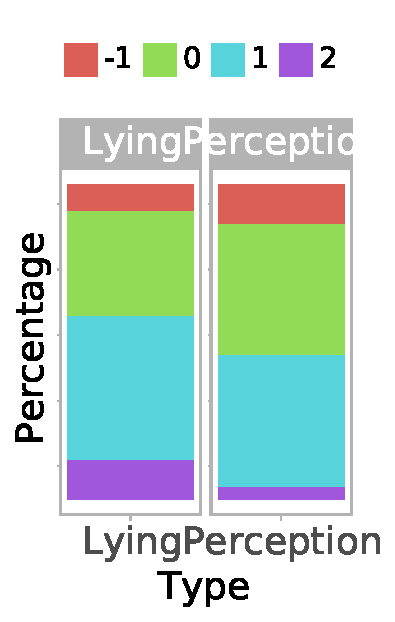
\includegraphics[width=\linewidth]{\autofig/DiploDemographics.pdf}
%	\caption{Most users self-assess themselves to be average or above at both lying and detecting lies.  Users assess themselves as better at perceiving lies than at telling them.}
%        \jbgcomment{I think this figure would be more efficient as normal text.  I'd cut.  Otherwise, change keys to something interpretable.}
%	\label{fig:questions2}
%\end{figure}
